% Working draft. Verify live course/template requirements before submission.
\documentclass[10pt,twocolumn,letterpaper]{article}
\makeatletter
\def\input@path{{../CVPR2026_模板源码/官方源码/}}
\makeatother
\usepackage[T1]{fontenc}
\usepackage[pagenumbers]{cvpr}
\usepackage{microtype}
\usepackage{amsmath}
\usepackage{booktabs}
\usepackage{graphicx}
\usepackage{tikz}
\usetikzlibrary{positioning,arrows.meta}
\definecolor{cvprblue}{rgb}{0.21,0.49,0.74}
\usepackage[breaklinks,colorlinks,allcolors=cvprblue]{hyperref}
\def\paperID{}
\def\confName{ARIN 5203 Working Draft}
\def\confYear{2026}
\title{Do AI Platform Agents Know What They Must Not Forget?\\
\large Compaction-Aware Intervention Before State-Changing Operations}
\author{Qingcheng Yu \quad Siu Kwun Yeung \quad Qingyin Guo\\
The Hong Kong University of Science and Technology}
\date{}
\begin{document}
\maketitle
\noindent\textbf{Working draft -- 31 October 2026.}
This manuscript is not submission-ready. Live template requirements, team
review, report-sharing preference, and final references require confirmation
before submission.

\begin{abstract}
An agent can preserve a user's goal while forgetting the evidence needed to
authorize its next tool call. We study this failure through a controlled,
course-scale evaluation of context retention and intervention before
state-changing operations. Twenty synthetic scenario families yield 60 matched
contexts: complete evidence, one critical deletion, and one word-matched noise
deletion. Six compressed strategies share a 384-token active-memory budget;
full history provides an unbudgeted reference. We compare direct model routing
with a deterministic audit that looks up the full proof record for every
source the compacted memory still cites. On eleven held-out families, typed proof memory
and several strong summaries all achieve 22/22 audited stable routes. Across
all 33 contexts, U-Fold-lite achieves 31/33 versus typed memory's 30/33. Typed
memory has perfect measured proof-source selection, but this metric does not
establish semantic entailment. Three upstream hold deletions still cause harmful
Execute routes; a separate deterministic registry test illustrates an
architectural response. Our contribution is an auditable integration of matched
perturbations, action-specific proof, repairability-aware routing, and regression
replay. A separate 24-context free-text diagnostic releases only Handoff,
revealing a brittle extraction interface rather than end-to-end readiness.
The main findings assume pre-existing authenticated records and external
lookup outside the active-memory budget; they do not certify production safety.
\end{abstract}

\section{Introduction}
An assistant is asked to reschedule a hotel booking. It finds an acceptable
price, checks availability, and delegates the change to a booking agent. Earlier
messages also contain an authorization limit and a hold requiring operator
review. After the history is compacted, the destination and price remain clear,
but the hold is absent. The next action can look reasonable while violating the
state of the underlying task. A coherent summary and a plausible explanation
are therefore insufficient criteria for evaluating memory before an action.
Compaction itself is unavoidable: self-attention cost grows quadratically
with sequence length and context windows are finite, so a long-running agent
must decide what its next step can still see. Our question is what that
decision does to the evidence behind a state-changing tool call.

The practical question is what evidence must remain available at a tool
boundary. Authorization has an actor, operation, target, scope, and validity
window. Policy clearance does not create authority; a requester cannot repair a
missing delegation simply by saying yes. A safe intervention policy must also
avoid unnecessary questions when valid evidence already permits execution.
These distinctions motivate our research question: under a fixed active-memory
budget, how do retention strategies and an action-specific evidence audit affect
Execute, Confirm, and Handoff decisions?

Our evaluation separates five choices: memory representation, critical versus
noise deletion, direct versus audited routing, token pressure, and the source
of authoritative records. This separation matters because improvement in one
layer can conceal a weakness in another. A conservative strategy may avoid
harm by losing all useful proof; a correct decision may cite a policy
requirement rather than an actual approval. Conversely, an audit may validate
everything it sees and still miss a hold that never reached its input.

We implement these comparisons in Agent Memory Crash Test, a research toolkit
and deterministic trace replay. Its contribution is an integration: a proposed
mutation has explicit proof obligations, matched evidence perturbations,
inspectable source references, and a released intervention route. A later
declared state transition makes the consequence visible in the replay. We do
not propose a new general-purpose summarizer, reproduce the full protocols of
the cited methods, or claim a state-of-the-art result.

The empirical conclusion is deliberately narrower than ``typed memory wins.''
Strong summaries tie on audited stable routing, and U-Fold-lite does better
across all held-out conditions. The useful findings concern which proof survives,
what the citation metric measures, and where validation stops helping. A
separate durable-record test supports treating conversational memory as a cache
and checking current authoritative proof beside the mutating tool.

\section{Related Work}
\paragraph{Memory and compaction.}
Mem2ActBench evaluates memory-grounded tool use rather than only explicit fact
retrieval; its main experiment supplies the correct tool to isolate parameter
grounding~\cite{mem2act}. U-Fold preserves a full archive and dynamically
constructs an evolving intent summary and task-relevant tool log~\cite{ufold}.
Our U-Fold-lite borrows that separation for a single checkpoint. ACON optimizes
compression guidelines using trajectory failures and distills
compressors~\cite{acon}; StateComp learns state-conditioned KEEP/READY routing
before summarizing eligible spans~\cite{statecomp}. We implement neither their
training nor their optimization procedures.

Governance Decay directly studies compaction-induced loss of in-context rules
and proposes Constraint Pinning~\cite{governance}. The Compaction Cliff is an
especially close method neighbor: Knowledge Triage already combines typed
retention, a deterministic post-compaction verifier, restoration or Unsafe
escalation, and downstream behavioral evaluation~\cite{cliff}. Those mechanisms
are established ideas. Our distinction is the application-specific proof
interface, retained-source reconstruction, and repairability-aware regression
contract; our implementation is not TypeCompact or its classifier.

PAIR restores the same environment checkpoint and repeatedly continues from
pre- and post-compression contexts, disabling later compression to isolate one
boundary's effect~\cite{pair}. It then adapts compression prompts. Our matched
deletions borrow a narrower local-comparison idea: they examine the next route
and do not estimate PAIR's terminal continuation effect or perform prompt
adaptation. A manual upstream deletion must not be described as an observed
compactor omission.

\paragraph{Intervention and stateful evaluation.}
AgentAbstain pairs should-act and should-abstain tasks, combining commit checks
with response judging for operational tasks~\cite{abstain}. Clarification and
refusal both count as abstention; our Confirm and Handoff instead encode
different repair permissions. HiL-Bench measures targeted assistance through
progressively discovered blockers and Ask-F1~\cite{hil}. DelegationBench
separates permission from missing information and shows gaps between judgment
and tool behavior~\cite{delegation}. We do not reproduce these benchmarks or
infer human preferences from our authored labels. Finally, $\tau$-bench evaluates
database outcomes and repeated-run reliability~\cite{tau}; ToolSandbox provides
state dependencies and intermediate trajectory checks~\cite{toolsandbox}.
These motivate consequence-aware evaluation, although our frozen main scores
use authored outcome flags rather than independent live-domain execution.

\section{Data and Evaluation Protocol}
\subsection{Synthetic action families}
The main benchmark contains twenty authored base families across platform
operations, financial-style evidence, and delegated travel/multi-agent
workflows. These are synthetic templates motivated by the team's experience,
not company incidents or production records. Each family fixes a proposed
action, runtime policy, source events, and canonical proof cards. Scenario
construction assigns the expected route and whether execution would be harmful.
Neither expected routes nor the unsafe-if-executed flag enters a model prompt.

Each base produces three siblings: complete evidence, removal of one
action-critical event, and removal of nearby irrelevant noise. Critical and
noise events share a role and word count and occupy adjacent positions. This
controls text removal approximately without claiming identical tokenizer
length. In particular, word matching is separate from the exact active-memory
token budget. The later reusable JSON contract and natural-language fixtures
require equal UTF-8 byte lengths; that stricter interface does not retroactively
make the main frozen experiment byte- or token-matched.

Nine families, comprising 27 contexts, support development. After the method,
prompts, thresholds, budget, and metrics were frozen, eleven separately
authored families supplied 33 held-out contexts. Their actors, actions, targets,
and identifiers differ from development. Siblings remain in the same split.
The held-out full-evidence routes include five Execute, three Confirm, and
three Handoff families. These are correlated variants of eleven scenarios,
not 33 independent deployment observations.

\subsection{What the intervention changes}
The deletion changes observable evidence while the authored underlying task
state remains fixed. Removing positive authority can require confirmation or
handoff. Removing a negative hold is different: the visible record can appear
clear even though execution remains prohibited in the authored world. These
cases test the limits of inference from missing observations. Noise deletion
provides the control for a route change caused merely by shorter text.

We define the \emph{stable subset} as complete-evidence and noise-deletion
contexts: 18 development and 22 held-out records per method. It is useful for
testing preserved behavior, but excludes critical deletions. We report both
stable and all-condition outcomes, including the hidden-hold failures. The
held-out run was performed once; subsequent interpretation checks do not
change its prompts, outputs, scores, or selection criteria.

\section{Method}
\subsection{Action-specific proof and routing}
An action is the tuple $a=(u,o,t,s,\tau)$: actor, operation, target, scope, and
effective time. A proof card supplies its type, source event identifiers,
issuer, subject, corresponding action fields, validity interval, authentication
flag, and transferability. The runtime policy declares trusted issuers and
required obligations. The main study assumes these records already exist and
are faithfully linked to their sources; it does not infer their authenticity
from ordinary text or verify real digital signatures.

\begin{table}[t]
\centering\small
\begin{tabular}{@{}p{0.26\columnwidth}p{0.67\columnwidth}@{}}
\toprule
Proof type & Distinct role \\
\midrule
Authority & Permission for this actor and action. \\
Clearance & Required policy checks have passed. \\
Active hold & An applicable blocker takes precedence. \\
Delegation & Permission is transferable to the acting agent. \\
Recovery & A required recovery path is evidenced. \\
Repair channel & A named authenticated responder can repair authority. \\
\bottomrule
\end{tabular}
\caption{Proof types are not interchangeable. ``No hold'' does not imply authority.}
\label{tab:types}
\end{table}

The validator filters cards by issuer, authentication, operation, target, scope,
and time. Authority must name the acting subject; delegation must also be
transferable. An applicable hold yields Handoff. Missing required clearance,
delegation, recovery, or non-repairable authority also yields Handoff. If all
requirements hold, verified authority yields Execute. Confirm is available
only when the sole authority gap has a valid repair channel and the remaining
obligations are satisfied. Confirm is therefore not a generic override button.

There is a deliberate closed-world limitation: without a visible applicable
hold, the local validator records the hold status as clear. It cannot tell
whether the source system has no hold or an upstream event was lost. The
registry test later changes the source of proof, not this logical inability
to recover an unseen fact.

\begin{figure}[t]
\centering
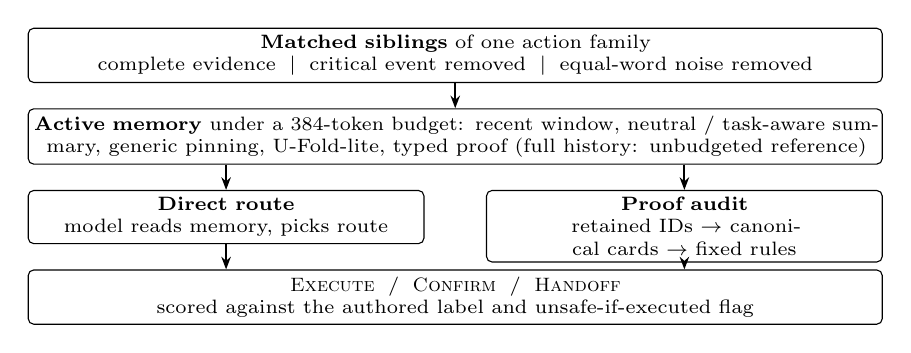
\begin{tikzpicture}[
  font=\scriptsize, node distance=3.2mm,
  box/.style={draw, rounded corners=2pt, align=center, inner sep=2.5pt, minimum height=5mm},
  arr/.style={-{Stealth[length=1.6mm]}, thick}]
\node[box, text width=0.88\columnwidth] (sib) {\textbf{Matched siblings} of one action family\\
complete evidence \;$\mid$\; critical event removed \;$\mid$\; equal-word noise removed};
\node[box, below=of sib, text width=0.88\columnwidth] (mem) {\textbf{Active memory} under a 384-token budget: recent window,
neutral / task-aware summary, generic pinning, U-Fold-lite, typed proof (full history: unbudgeted reference)};
\node[box, anchor=north west, text width=0.40\columnwidth] (dir) at ([yshift=-3.2mm]mem.south west) {\textbf{Direct route}\\model reads memory, picks route};
\node[box, anchor=north east, text width=0.40\columnwidth] (aud) at ([yshift=-3.2mm]mem.south east) {\textbf{Proof audit}\\retained IDs $\rightarrow$ canonical cards $\rightarrow$ fixed rules};
\node[box, anchor=north west, text width=0.88\columnwidth] (route) at ([yshift=-3.2mm]dir.south west) {\textsc{Execute} \;/\; \textsc{Confirm} \;/\; \textsc{Handoff}\\
scored against the authored label and unsafe-if-executed flag};
\draw[arr] (sib) -- (mem);
\draw[arr] (mem.south -| dir.north) -- (dir.north);
\draw[arr] (mem.south -| aud.north) -- (aud.north);
\draw[arr] (dir.south) -- (dir.south |- route.north);
\draw[arr] (aud.south) -- (aud.south |- route.north);
\end{tikzpicture}
\caption{Evaluation pipeline. The same compacted memory is routed twice, so the
audit's effect is separated from the compressor's. The budget applies to active
memory only; canonical records are looked up outside it.}
\label{fig:architecture}
\end{figure}

\subsection{Representations and budget enforcement}
Six compressed strategies share the same raw-Qwen-token limit. Recent window
retains recent events; generic pinning prioritizes events using generic textual
cues. Neutral and task-aware summaries use different instructions but the
same output interface. U-Fold-lite emits an intent summary and source-linked
proof log. Typed proof memory deterministically serializes visible cards into
compact capsules. Full history is an unbudgeted information reference, not a
guaranteed performance ceiling.

Typed capsules contain source/card identifiers, type, issuer, subject,
authentication and transferability, plus \emph{action-scope-match} and
\emph{valid-now} bits computed from canonical fields and the proposed action.
They do not repeat full targets, scopes, and timestamps on every line. These
are action-dependent, precomputed features, not evidence that a model learned
to extract or reason over the omitted raw fields. No expected route or unsafe
label is used to compute them. Their convenience is part of the representation
being evaluated and an important limit on claims about compression alone.

The budget builder counts the final active text using the target local
tokenizer, trims overlong drafts, and fills remaining space using only neutral
events. Protected proof cannot be reintroduced by fill. The utilization floor
is $\lceil0.9\times384\rceil=346$ tokens, preventing an empty conservative
memory from winning by consuming almost no context. The router receives the
same action and policy separately and is blinded to method identity. Shared
instructions, the repeated allowed-source list, external storage, and lookup
cost are not included in the 384-token memory limit; the complete routing
prompt is larger.

\subsection{Direct route versus canonical audit}
The direct model emits a route, cited event identifiers, and missing
obligations. Parsing rejects invisible or duplicate identifiers and invalid
formats; malformed output releases Handoff. The deterministic audit uses the
same memory's retained source set. A canonical card is available when all of
its source identifiers survive. The audit then validates the reconstructed
record rather than treating summary prose or the model's proposed route as
authority. Consequently, a surviving identifier can unlock a complete external
record even when the active summary paraphrases it incorrectly. This is
retention plus lookup, not self-contained proof compression.

\subsection{Metrics and reporting units}
Route accuracy compares the released route with its authored label. Harmful
Execute is the conjunction of an Execute route and the authored
unsafe-if-executed flag. Unnecessary intervention means withholding execution
when the expected route is Execute. Safe-autonomy recall uses eligible Execute
cases. Main frozen records do not independently execute real bookings,
transfers, or deployments; subsequent replay applies a declared transition.

Visible-card recall measures which cards supplied to the compactor remain
recoverable through retained sources. Critical retention concerns critical
evidence that was supplied, not an ability to reconstruct an event deleted
before compaction. Noise invariance checks paired routes. Audit helpfulness
and harmfulness count corrected and spoiled direct decisions.

The frozen citation metric is a macro-average. For record $i$, let $C_i$ be
parsed citations and $V_i$ the visible canonical proof-source identifiers.
For nonempty $C_i$, $p_i=|C_i\cap V_i|/|C_i|$, and the reported value is
$n^{-1}\sum_i p_i$. A zero-citation Handoff receives 1 under the frozen
convention; another zero-citation route receives 0. This measures selection
of any proof source, not entailment, relevance to the decisive obligation,
or completeness of authorization. We retain that definition rather than
retroactively replacing it with a citation-weighted average.

\section{Experiments and Results}
\subsection{Execution and provenance}
The main held-out comparison uses local Ollama \texttt{qwen3.5:9b}, temperature 0,
seed 5203, and versioned prompts. The held-out run generated 99 compactor and
231 router outputs, plus one separate warm-up. It completed 330 measured
generations in 6,189.49 seconds, recording 337,432 input and 33,564 output
tokens. The manifest separately records 2,001 tokenizer probes; those probes
are not additional independent task evaluations. External API fees were zero.
Budget, provenance, neutral-fill, blinding, and format gates passed. Passing
instrumentation establishes that the intended comparison ran, not that its
semantic assumptions are universally valid.

Each result prefix owns immutable raw, summary, audit, and manifest files.
The raw trace records model-visible inputs and outputs; the summary supplies
scores, the audit supplies protocol checks, and the manifest supplies model,
configuration, hashes, timing, and usage. Table~\ref{tab:provenance} identifies
the main bundles in the course repository.\footnote{Research archive:
\url{https://github.com/Qingthefish/arin5203-agent-intervention}.
Prefixes resolve under the results directory linked from the repository's
technical README.}
The experiment index is discovery metadata. Presentation metrics are derived
views and do not replace the frozen records.

\begin{table*}[t]
\centering\small
\begin{tabular}{@{}lrrrrrr@{}}
\toprule
 & \multicolumn{2}{c}{Stable correct /22} & All correct /33 & \multicolumn{2}{c}{Harmful Execute /33} & Unnecessary \\
Method & Direct & Audit & Audit & Direct & Audit & Audit \\
\midrule
Full history$^*$ & 14 & 22 & 30 & 14 & 3 & 0 \\
Recent window & 6 & 6 & 15 & 0 & 0 & 10 \\
Neutral summary & 11 & 22 & 30 & 16 & 3 & 0 \\
Task-aware summary & 10 & 22 & 30 & 18 & 3 & 0 \\
Generic pinning & 10 & 6 & 15 & 18 & 0 & 10 \\
U-Fold-lite & 14 & 22 & 31 & 14 & 2 & 0 \\
Typed proof & 14 & 22 & 30 & 7 & 3 & 0 \\
\bottomrule
\end{tabular}
\caption{Frozen held-out routing. Stable means complete/noise-deletion contexts;
all-condition results include critical deletions. Harmful Execute uses authored
unsafe flags, not independent live-domain outcomes. $^*$Unbudgeted reference.
The six compressed methods share a 384-token active-memory limit.}
\label{tab:main}
\end{table*}

\begin{table*}[t]
\centering\small
\begin{tabular}{@{}p{0.53\textwidth}p{0.40\textwidth}@{}}
\toprule
Artifact prefix & Evidence role \\
\midrule
\path{typed_exact_budget_heldout_qwen_v1} & Frozen seven-method comparison; raw, summary, audit, manifest. \\
\path{typed_budget_sweep_dev_qwen_v1} & Development sensitivity; replayed compactor outputs and new routes. \\
\path{durable_proof_store_deterministic_v1} & Deterministic architecture test with authenticated-record assumptions. \\
\path{nl_extraction_dev_diagnostic_qwen_v1} & Development-only extraction diagnostic; JSON-mode interface failure. \\
\path{heldout_bootstrap_ci_v1} & Post-hoc family-clustered intervals derived from the frozen held-out trace; zero model calls. \\
\bottomrule
\end{tabular}
\caption{Compact provenance map. Historical negative gates are identified in the
text; they are not pooled with held-out samples.}
\label{tab:provenance}
\end{table*}

\subsection{Main comparison: safety and autonomy together}
\begin{figure}[t]
\centering
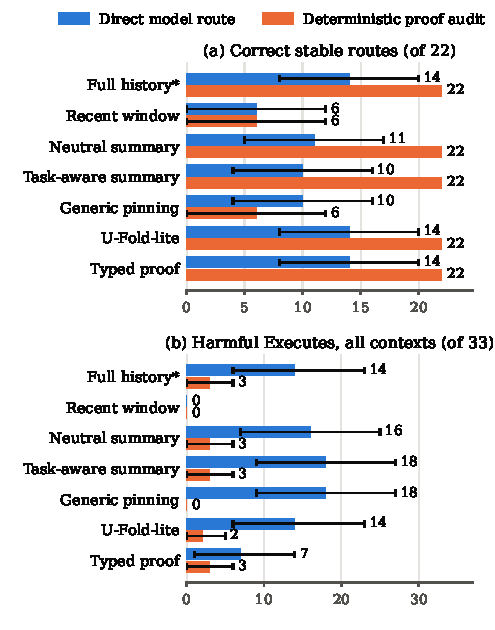
\includegraphics[width=\columnwidth]{figures/heldout_direct_vs_audit.pdf}
\caption{Held-out routing per memory strategy. Blue: the model's direct route;
orange: the same memory after the deterministic proof audit. Bars show frozen
counts; whiskers are family-clustered 95\% bootstrap intervals over the eleven
held-out families (no whisker when every resample gives the same count).
$^*$Full history is an unbudgeted reference.}
\label{fig:heldout}
\end{figure}

Table~\ref{tab:main} and Figure~\ref{fig:heldout} show why a single success percentage is insufficient.
Typed memory plus audit achieves 22/22 correct stable routes, with no stable
harmful Execute, unnecessary intervention, or noise-induced route change.
Direct routing on that memory achieves 14/22 and four stable harmful Executes.
Across all 33 contexts, the audit corrects ten typed direct errors and spoils
none; seven direct harmful Executes become three after audit.
Resampling the eleven held-out families with replacement (siblings kept
together, 10{,}000 draws) gives a descriptive sense of this variability: the
audit adds 8 correct stable typed routes (95\% interval 2--14) and removes
4 harmful typed Executes (0--10). The harm reduction is larger for the neutral
and task-aware summaries, 13 (6--21) and 15 (7--23), because their direct routes
executed more often. Perfect audited scores yield degenerate intervals; with
eleven correlated families, none of these intervals is a significance test.

However, neutral summary, task-aware summary, and U-Fold-lite also achieve
22/22 audited stable routes. Across all conditions, U-Fold-lite reaches 31/33,
compared with 30/33 for typed memory and both summaries. Its loss of additional
positive evidence causes conservative blocking in one hidden-hold case. This
avoids harm without recovering the missing hold. It is a real outcome of this
test and prevents a universal typed-superiority interpretation.

Recent-window and generic-pinning audits avoid harmful Execute but retain no
eligible safe autonomy and produce ten unnecessary interventions each. Generic
pinning's audit also spoils ten direct decisions while correcting fifteen.
These results distinguish useful restraint from indiscriminate withholding.
An evidence checker cannot preserve autonomy if the memory no longer supplies
required positive proof.

\subsection{Source selection is not entailment}
\begin{table}[t]
\centering\small
\setlength{\tabcolsep}{2pt}
\begin{tabular}{@{}lrrr@{}}
\toprule
Method & Card recall & Macro source & Proof / cited \\
 & (\%) & selection (\%) & occurrences \\
\midrule
Full history & 100.0 & 98.2 & 100/103 \\
Recent window & 0.0 & 45.5 & 0/18 \\
Neutral summary & 100.0 & 75.7 & 110/167 \\
Task-aware & 100.0 & 69.1 & 108/190 \\
Generic pinning & 67.0 & 84.8 & 75/93 \\
U-Fold-lite & 99.0 & 98.2 & 101/104 \\
Typed proof & 100.0 & 100.0 & 112/112 \\
\bottomrule
\end{tabular}
\caption{All-condition evidence metrics. Last-column counts are a post-hoc
recount of parsed citation occurrences; the middle column preserves the frozen
macro convention, including zero-citation Handoff scores.}
\label{tab:source}
\end{table}

Table~\ref{tab:source} separates retention from direct-router source selection.
Typed proof achieves 100\% on both measured quantities. This supports
inspectability under the card assumption, not independent verification of a
free-text argument. A post-hoc recount across all seven methods finds that all
787 parsed citation occurrences are inside their respective active source sets.
Lower summary precision therefore cannot be described as citing nonexistent
events. It includes selection of visible policy or noise sources that are not
canonical proof-card sources. The recent window's 45.5\% macro score despite
zero proof-source citations also exposes the empty-Handoff convention.

An existing source can still be misinterpreted. In neutral summary's
\texttt{held-z3::remove\_action\_critical} record, the summary asserts confirmed
authority although the canonical visible records contain no authority card.
The audit withholds execution. This trace illustrates three separate questions:
does the source exist, does it support the stated claim, and does the complete
current action have sufficient proof? Our citation statistic directly answers
only a source-selection question.

\subsection{Boundary cases and durable proof}
The typed audit handles all eight non-hold critical deletions by withholding
execution. These gaps are not all repairable with one answer: missing delegation
or recovery can require Handoff. The remaining three critical deletions remove
an active hold before the compactor sees the history. All three retain harmful
Execute outcomes. Perfect retention of supplied cards and perfect local
validation cannot establish completeness of upstream observations.

A separate development-only test therefore queries a point-in-time canonical
registry before validating the action. Three new families each have six
conditions: recover a hold, ignore an expired hold, ignore a revoked hold,
recover authority, reject wrong-scope authority, and reject revoked authority.
Memory-only routing is correct on 12/18 cases with three harmful Executes;
registry-assisted routing reaches 18/18 with none. Six route changes help and
none harm, while twelve controls remain unchanged. This zero-model
demonstration assumes authenticated external records and validates them through
the same checker. It does not measure distributed consistency, service latency,
or production authorization reliability.

\subsection{Development budget sensitivity}
\begin{table}[t]
\centering\small
\begin{tabular}{@{}lrrr@{}}
\toprule
Audited stable routes /18 & 384 & 256 & 192 tokens \\
\midrule
Recent window & 6 & 6 & 6 \\
Neutral summary & 18 & 18 & 18 \\
Task-aware summary & 18 & 18 & 18 \\
Generic pinning & 6 & 6 & 6 \\
U-Fold-lite & 17 & 17 & 15 \\
Typed proof & 18 & 18 & 18 \\
\bottomrule
\end{tabular}
\caption{Development sensitivity, not a second held-out evaluation. Frozen
compactor outputs are rebudgeted; routes at 256/192 tokens are newly generated.}
\label{tab:budget}
\end{table}

The sweep first reconstructs the 384-token development memories from frozen
compactor outputs and checks text hashes, exact counts, sources, fill, and
format against the original run. It then generates 324 router outputs at
256 and 192 tokens; it does not rerun summary generation. Table~\ref{tab:budget}
shows that strong summaries and typed proof retain 18/18 audited stable routes
at the tightest budget. Stable-subset visible-card recall falls to 97.8\% for
typed proof because two contexts lose one non-decisive recovery card; generic
pinning's stable-subset recall falls to 26.3\%.
These observations characterize this implementation's sensitivity, rather than
proving typed accuracy dominance or measuring how a newly prompted compressor
would adapt to each budget.

\subsection{Negative gates that changed the design}
Two development failures explain the final interface. In
\path{audit_increment_qwen_v2}, direct routing is correct on 4/9 contexts, a
generic critic on 2/9, and candidate-visible evidence review on 3/9. The critic
spoils three of four initially correct decisions; evidence review retains two
harmful Executes. Asking a second model to reconsider the same conclusion
therefore did not supply a reliable proof boundary.

In \path{blind_proof_qwen_v1}, hiding the candidate decision improves routing
from 4/9 to 8/9, yet a verifier treats clearance as authority and still releases
a harmful Execute. Four format failures also reveal an interface contradiction
around empty citations for UNKNOWN. These are development diagnostics, not
additional held-out comparisons. They motivate distinct evidence types and a
deterministic mapper, while warning against interpreting a high routing score
or parser fallback as a general reasoning capability.

\subsection{Natural-language diagnostic: a brittle upstream interface}
The main study does not test card creation. A frozen extension selects four
existing development families, all three siblings, and clean/distractor
variants: 24 contexts, with no compactor comparison. The selection covers
three domains, original route categories, and three distractor styles, not
every domain-by-route cell. Literal fields and source quotes pass to the fixed
validator; invalid distractors should be extracted faithfully and then rejected.
The run completes all 24 calls in 1,782.22 seconds, using 42,498 input and 25,432
output tokens at zero external API fee. Source, prompt, dataset and scoring
hashes were frozen before generation; recording checks pass, with no retuning.

All 24 released routes are Handoff: 10/24 agree with world-gold and 8/24 with
the visible-evidence oracle. All eight eligible Execute cases are withheld,
and six expected Confirm routes become Handoff. Nineteen outputs violate the
strict extraction contract. Macro literal-card exact recall is 11.5\%; the
158/170 matched-field score is conditional on only 17 parsed cards out of 94
declared literal cards, not overall extraction accuracy. A post-hoc raw review
finds 93 claim occurrences at declared sources; 76 are rejected for nonstring
scope values. Most post-parser omissions are therefore contract rejection, not
missing source recognition. Zero harmful Execute,
zero accepted distractors and invariant noise routes do not establish useful
safety discrimination when every action is withheld.

Raw review finds numeric scope values where the contract requires strings,
plus subjects confused with the acting agent or an operation phrase. For
example, record \texttt{D8-03} in the distractor/full condition names an
authorized responder, but the extracted subject is the acting agent.
Authentication needs
separate caution: some synthetic messages say only ``signed,'' while their
canonical gold marks authentication successful. The prompt asks for explicit
verification, so conservative false flags can reflect a wording ambiguity.
These canonical mismatches are not all evidence of a model mistake.

This is a negative result for the frozen extraction-and-validation interface,
not arbitrary prose extraction or schema-constrained decoding. The client
requests JSON-object mode; Ollama's schema-constrained option is a distinct
mechanism~\cite{ollama-schema}. The result does not alter the original held-out
scores, and no automatic follow-up run is performed. It narrows the engineering
claim: a validator for supplied proof cards is not a reliable text-to-proof
system by itself.

\section{Limitations and Developer Implications}
The benchmark is small, synthetic, risk-enriched, and evaluated with one local
model and one generation per context. Shared siblings and method outputs
preclude treating record counts as independent evidence of broad generalization.
The authored policies and proof cards make the audit tractable but leave
real-world extraction, semantic ambiguity, trust establishment, and malicious
issuers unresolved. Quote containment in the extension confirms a substring,
not entailment or signature validity. Authentication flags in synthetic
records must not be mistaken for real cryptographic checks.

The budget comparison concerns active memory. Canonical rehydration,
precomputed action-match bits, and shared unbudgeted inputs provide information
and computation beyond compressed text alone. Their storage, lookup, and
availability costs require separate accounting in a deployed system. Likewise,
the frozen harmful-Execute metric uses an authored flag, and the replay applies
a declared transition. Neither measures an independent real-world outcome.
Confirm and Handoff are route semantics, not a measured human workflow or
evidence that intervention burden is acceptable to users.

The reusable toolkit expresses mutation, obligations, matched deletions, and
retained-source snapshots as a JSON contract and emits JSON/JUnit reports.
Those report formats and CI gates are ordinary engineering choices, already
supported by evaluation tools such as Promptfoo and DeepEval~\cite{promptfoo,deepeval}.
The reference proof-source selector assumes author-declared cards; it is not a
learned extractor. A replay and a passing suite should support regression
investigation, not a production-readiness claim.

A developer can nevertheless follow a concrete procedure. First enumerate
mutating tools and bind proof to exact arguments. Next keep permissions,
holds, and revocations on an authoritative path distinct from chat summaries.
At execution time, validate issuer, scope, time, delegation, and recovery, then
choose intervention according to who can repair the missing obligation.
Finally replay complete, critical-deletion, and matched-noise contexts whenever
the model, memory policy, or prompt changes. Compression timing, evidence
storage, and execution permission are separate decisions; a summary is not an
authorization database.

\section{Conclusion}
This project provides a controlled action-evidence test contract and an
inspectable implementation at course scale. Deterministic auditing repairs
many direct-route mistakes when sufficient source-linked proof survives,
while strong summaries remain competitive and upstream hold loss remains a
hard boundary. The strongest supported lesson is to preserve or revalidate
the evidence required by the next action, and evaluate its availability,
interpretation, and completeness separately. Extending that lesson to arbitrary
text or deployed systems requires evidence beyond this study.

{\small
\begin{thebibliography}{15}
\bibitem{mem2act}
Yiting Shen, Kun Li, Wei Zhou, and Songlin Hu.
Mem2ActBench: A Benchmark for Evaluating Long-Term Memory Utilization in
Task-Oriented Autonomous Agents. arXiv:2601.19935, 2026.
\url{https://arxiv.org/abs/2601.19935}.

\bibitem{ufold}
Jin Su, Runnan Fang, Yeqiu Li, Xiaobin Wang, Shihao Cai, Pengjun Xie,
Ningyu Zhang, and Fajie Yuan.
U-Fold: Dynamic Intent-Aware Context Folding for User-Centric Agents.
In \emph{Findings of ACL}, 2026.
\url{https://aclanthology.org/2026.findings-acl.897/}.

\bibitem{acon}
Minki Kang, Wei-Ning Chen, Dongge Han, Huseyin A. Inan, Lukas Wutschitz,
Yanzhi Chen, Robert Sim, and Saravan Rajmohan.
ACON: Optimizing Context Compression for Long-horizon LLM Agents.
In \emph{ICML}, 2026.
\url{https://proceedings.mlr.press/v306/kang26b.html}.

\bibitem{statecomp}
Mingxuan Wang et al.
StateComp: Learning When to Compress History in Long Horizon Agents.
arXiv:2609.27298, 2026.
\url{https://arxiv.org/abs/2609.27298}.

\bibitem{governance}
Shiyang Chen.
Governance Decay: How Context Compaction Silently Erases Safety Constraints
in Long-Horizon LLM Agents. arXiv:2606.22528, 2026.
\url{https://arxiv.org/abs/2606.22528}.

\bibitem{cliff}
Saber Zerhoudi, Jelena Mitrovi\'c, and Michael Granitzer.
The Compaction Cliff in Long-Running AI Agent Memory.
In \emph{CIKM}, 2026.
\url{https://arxiv.org/abs/2608.22752}.

\bibitem{pair}
Guanghui Min et al.
Adapting Context Compression for Long-Horizon Agents with Counterfactual
Continuations. arXiv:2609.36526, 2026.
\url{https://arxiv.org/abs/2609.36526}.

\bibitem{abstain}
Xun Liu et al.
AgentAbstain: Do LLM Agents Know When Not to Act?
arXiv:2607.10059, 2026.
\url{https://arxiv.org/abs/2607.10059}.

\bibitem{hil}
Tu Trinh et al.
HiL-Bench (Human-in-Loop Benchmark): Do Agents Know When to Ask for Help?
arXiv:2604.09408, version 4, 2026.
\url{https://arxiv.org/abs/2604.09408}.

\bibitem{delegation}
Shiva Pochampally.
DelegationBench: Measuring When AI Agents Should Ask Before Acting.
arXiv:2610.05532, 2026.
\url{https://arxiv.org/abs/2610.05532}.

\bibitem{tau}
Shunyu Yao, Noah Shinn, Pedram Razavi, and Karthik Narasimhan.
$\tau$-bench: A Benchmark for Tool-Agent-User Interaction in Real-World Domains.
arXiv:2406.12045, 2024.
\url{https://arxiv.org/abs/2406.12045}.

\bibitem{toolsandbox}
Jiarui Lu et al.
ToolSandbox: A Stateful, Conversational, Interactive Evaluation Benchmark
for LLM Tool Use Capabilities. arXiv:2408.04682, 2024.
\url{https://arxiv.org/abs/2408.04682}.

\bibitem{promptfoo}
Promptfoo. Output Formats. Official documentation, accessed 23 October 2026.
\url{https://www.promptfoo.dev/docs/configuration/outputs/}.

\bibitem{deepeval}
DeepEval. Unit Testing in CI/CD. Official documentation, accessed 23 October 2026.
\url{https://deepeval.com/docs/evaluation-unit-testing-in-ci-cd}.

\bibitem{ollama-schema}
Ollama. Structured Outputs. Official documentation, accessed 23 October 2026.
\url{https://docs.ollama.com/capabilities/structured-outputs}.
\end{thebibliography}
}
\end{document}
